\documentclass[onecolumn]{IEEEtran}
\usepackage[utf8x]{inputenc}
\usepackage{graphicx}
\usepackage{times}
\usepackage[tbtags]{amsmath}
\usepackage{cite}
\usepackage[all]{xy}
\usepackage{subfigure}
\usepackage{wrapfig}
\usepackage{multicol}
\usepackage{cite}
\usepackage{url}
\usepackage[tbtags]{amsmath}
\usepackage{amsmath,amssymb,amsfonts,amsbsy}
\usepackage{bm}
\usepackage{algorithm}
\usepackage{algorithmic}
\usepackage[all]{xy}
\usepackage[centerlast, small]{caption}
\usepackage[colorlinks=true, citecolor=blue, linkcolor=blue, urlcolor=blue, breaklinks=true]{hyperref}
\begin{document}
\title{Informe de Matlab}
\author{David Ricardo Martínez Hernández Código: $261931$}
\maketitle
\markboth{Universidad Nacional de Colombia}{}{}
\floatname{algorithm}{Algoritmo}
\section{Primer Punto}
\subsection{Parte A}
\noindent
La ecuación establecida para este punto se resolvió la ecuación de diferencias de la ecu.\ref{ecu1}, tomado como condiciones iniciales $y\left[ -1 \right]=y\left[ -2 \right]=0$.
\begin{equation}\label{ecu1}
y\left[ n \right] =  - a_1 \left[ {yn - 1} \right] - a_2 y\left[ {n - 2} \right] + b_0 x\left[ n \right]
\end{equation}
\noindent
El comando utilizado para calcular la respuesta impulso de la ecu.\ref{ecu1} fue \textbf{filter(b,a,X[n])}. Este comando pide los coeficiente de la ecuación de diferencias como lo muestra la ecu.\ref{ecu2}, estos valores se deben ingresar de la siguiente manera
\begin{verbatim}
Ingrese los coeficientes del sistema, que acompañan a la Y[n]:
[a1 a2 a3 a4 a5 a6 . . . an]
Ingrese los coeficientes del sistema, que acompañan a la X[n]:
[b1 b2 b3 b4 b5 b6 . . . bn]
\end{verbatim}
\noindent
no importa si son de la misma longitud o no, se debe tener en cuenta el orden en el que se ingresan, para poder calcular bien la respuesta impulso del sistema.
\begin{equation}\label{ecu2}
    \sum\limits_{k = 0}^N {a_{k + 1} y_{n - k}  = \sum\limits_{k = 0}^M {b_{k + 1} x_{n - k} \ \ \ \ \ \ \ \ \ \ 1 \le n \le P} }
\end{equation}
para poder limitar la salida de la respuesta impulso de $0 \le n \le 19$, se utilizo el siguiente condicional, por si $h[n]$ es mayor a dicho valor lo corrige para que solo muestre los $50$ primeros datos (el $.*ones(1,50)$ se utilizó para asegurar que el vector quedara de $50$ posiciones).
\begin{verbatim}
if (length(y)>=1 && length(y)<=50)
	y=y;
else(length(y)>=51);
    y=y(1:50).*ones(1,50);
end
\end{verbatim}
\noindent
La salida de esta respuesta impulso se encuentra representada por la figura$(1)$, en la parte inferior y en la parte superior se encuentra el gráfico de la entrada determinada por el usuario, este vector se ingresa de la siguiente manera: $[x_0 \ \ x_1 \ \ x_2\ \ . \ \ . \ \ . \ \ x_6 \ \ x_{50}]$.\\
Para la respuesta paso se utilizo el siguiente código
\begin{verbatim}
l=input('Ingrese el máximo valor de la función U[n]: \n');
u=[1,ones(1,l)];
y1=filter(b,a,u);
z1=(conv(u,y1,'full'));
\end{verbatim}
\noindent
para poder graficar la respuesta paso para $0 \le n \le 100$ se utilizó el siguiente código
\begin{verbatim}
if (length(z1)>=1 && length(z1)<=101)
	figure(3),
	stem(0:length(z1)-1,z1,'gx'),
    hold
    legend('conv(U1[n],h1[n])'),
else(length(z1)>=102)
	z1=z1(1:102).*ones(1,102);
	figure(3),
	stem(0:101,z1,'gx');
    hold
    legend('conv(U1[n],h1[n])'),
end
\end{verbatim}

\subsection{Parte B}
\noindent
Se definió una respuesta impulso $h_2[n]$ descrita por la ecu.\ref{ecu3}
\begin{equation}\label{ecu3}
h_2 \left[ n \right] = \left\{ \begin{array}{l}
 h\left[ n \right] \ \ \ \ 0 \le n \le 5 \\
 0 \ \ \ \ \ \ \ \ otros \ \ valores \\
 \end{array} \right.    
\end{equation}
\noindent
Esta respuesta impulso se definió de la siguiente manera
\begin{verbatim}
if (length(y)>=1 && length(y)<=20)
	h2=y;
else(length(y)>=20)
	h2=y(1:20).*ones(1,20);
end
\end{verbatim}
\noindent
para calcular la salida del nuevo sistema con dicha respuesta impulso se calculo con la ecu.\ref{ecu4} se utilizo
\begin{equation}\label{ecu4}
    y_2\left[ n \right] = x_2 \left[ n \right]*h_2 \left[ n \right]
\end{equation}
\begin{verbatim}
xn2 = input('Introducir el valor del vector X[n] para la parte B: \n');
z2=conv(xn2,h2,'full');
if (length(z2)>=1 && length(z2)<=20)
	figure(4),
	stem(0:19,z2,'yo'),
    hold
    legend('conv(X2[n],h2[n])'),
else(length(y)>=20)
	z2=z2(1:20).*ones(1,20);
	figure(4),
	stem(0:19,z2,'yo'),
    hold
    legend('conv(X2[n],h2[n])'),
end
\end{verbatim}
\noindent
Para calcular la respuesta al escalón unitario del nuevo sistema $y_2\left[ n \right]$ se calculo mediante
\begin{verbatim}
l2=input('Introdusca el maximo valor de la funcion U[n] para el punto B: \n');
u2=[1,ones(1,l2)];
z3=(conv(u2,h2,'full'));
n3=0:length(z3)-1;
if (length(z3)>=1 && length(z3)<=100)
	figure(5),
	stem(n3,z3,'r+'),
    hold
    legend('conv(U2[n],h1[n])'),
else(length(z3)>=101)
    z3=z3(1:101).*ones(1,101);
    figure(5),
    stem(0:100,z3,'r+'),
    hold
    legend('conv(U2[n],h2[n])'),
end
\end{verbatim}

\subsection{Parte C}
\noindent
Para poder ejecutar el programa se escribe en la ventana de comandos de Matlab \textit{punto1\_1} o \textit{punto2\_1}.
\begin{figure}[]
    \begin{minipage}[t]{1cm}
    \centering
        \subfigure[Respuesta paso para el primer sistema]{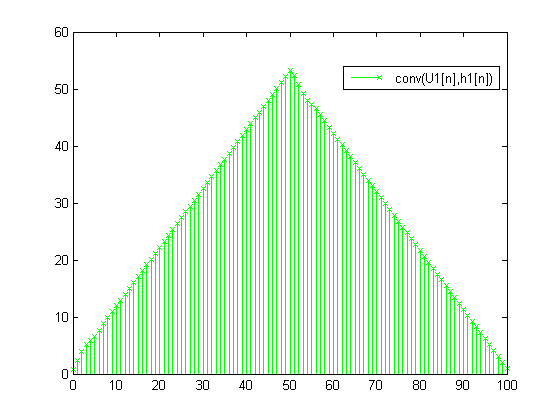
\includegraphics[scale=0.65]{steep1.png}}
    \end{minipage}
    \hfill\begin{minipage}[t]{9cm}
    \centering
        \subfigure[Respuesta paso para el segundo sistema]{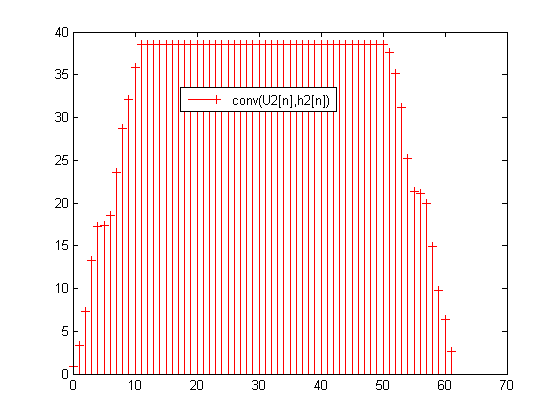
\includegraphics[scale=0.65]{steep2.png}}
    \end{minipage}
            \label{fig2}
\end{figure}
\noindent
Para esta respuesta se definió el vector \verb'xn=[1 2 3 5 2 1 4 5 2 3 5 2]' para el primer vector solicitado, para la ecuación de diferencias \verb'a=[1 0.8 0.64]' y \verb'b=[0.866 0 0]', el paso se definió \verb'l=50 u=[1,ones(1,l)]' y la gráfica que se obtiene es la figura $(a)$, luego se ingreso el vector \verb'xn2=[1 2 3 5 2 1 4 5 2 3 5 2]' y la respuesta impulso \verb'h2'(descrita anteriormente) y la señal paso por \verb'l2=50 u2=[1,ones(1,l2)]'.\\
Como los dos sistemas son completamente diferentes la respuesta paso también debe ser diferente, aunque se halla definido una respuesta impulso para el sistema $2$ igual a la del sistema $1$ pero como su tamaño es diferente la respuesta paso es diferente la una de la otra.\\
Como el primer es una ecuación de diferencias su respuesta impulso es recursiva, es decir siempre va a crecer porque depende de sus valores anteriores e ira creciendo, para este caso en particular.\\
\textbf{Estos programas pueden calcular las soluciones para cualquier valor que se ingrese en los datos de entrada}, ya sea un impulso en la entrada o un vector muy complejo.

\section{Segundo Punto}
\noindent
Los siguientes sistemas son los utilizados para calcular la respuesta impulso mostrado en la Figura \ref{fig1}.\\
$S_1$: $h_1 \left[ n \right] = \left\{ \begin{array}{l} \left( {\frac{1}{2}} \right)^n  \ \ \ \ 0 \le n \le 5 \\ \ \ 0 \ \ \ \ \ \ \ otros \ \ valores \\ \end{array} \right.$\\
$S_2$: $h_2 \left[ n \right] = \left\{ \begin{array}{l} 1 \ \ \ \ \ \ \ 0 \le n \le 5 \\ 0 \ \ \ \ \ \ \ otros \ \ valores \\ \end{array} \right.$\\\\
$S_3$: $y_3 \left[ n \right] = \frac{1}{4}x\left[ n \right] + \frac{1}{2}x\left[ {n - 1} \right] + \frac{1}{4}x\left[ {n - 2} \right]$\\\\
$S_4$: $y_4 \left[ n \right] = \frac{9}{{10}}y\left[ {n - 1} \right] - \frac{4}{5}y\left[ {n - 2} \right] + x\left[ n \right] + x\left[ {n - 1} \right]$\\
\begin{figure}[H]
	\centering
		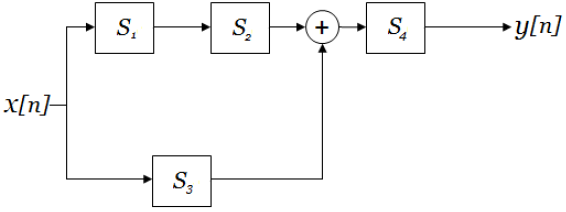
\includegraphics[scale=0.6]{sys.png}
	\caption{Sistema para calcular la respuesta impulso}
    \label{fig1}
\end{figure}
\noindent
Para definir los sistemas $S_3$ y $S_4$ se utilizo el siguiente código
\begin{verbatim}
%S3 definición del sistema 3
x1=input('Ingrese el valor del vector X[n] para el sistema S3:: \n');
a1 =input('Ingrese los coeficientes del sistema, que acompañan a la Y[n] para el sistema S3: \n');
b1 = input('Ingrese los coeficientes del sistema, que acompañan a la X[n] para el sistema S3: \n');
h3 = filter(b1, a1, x1);
%S4 definición del sistema 4
x2=input('Ingrese el valor del vector X[n] para el sistema S4: \n');
a2 = input('Ingrese los coeficientes del sistema, que acompañan a la Y[n] para el sistema S4: \n');
b2 =input('Ingrese los coeficientes del sistema, que acompañan a la X[n] para el sistema S4: \n');
h4 = filter(b2, a2, x2);
\end{verbatim}
\noindent
Como el tamaño de la convolución entre $S_1$ y $S_2$ puede ser mayor que la respuesta impulso de $S_3$, se deben igualar los tamaños de los vectores para poder sumarlos punto a punto, esto se logro de la siguiente manera
\begin{verbatim}
%Convolución de los sistemas S1 y S2
c1=conv(h1,h2,'full');
%suma de la convolución anterior con S3
if(length(h3)==length(c1));
	c1=c1;
	h3=h3;
	elseif(length(h3)<length(c1));
	c1=c1(1:length(h3)).*ones(1,length(h3));
	h3=h3;
	elseif(length(h3)>length(c1))
	c1=c1;
	h3=h3(1:length(c1)).*ones(1,length(c1));
end
s=h3+c1;
\end{verbatim}
\noindent
Finalmente al obtener la respuesta impulso producida por la combinación de $S_1$, $S_2$ y $S_3$, se hace la convolución con $S_4$ de la siguiente manera
\begin{verbatim}
%convolución de lo anterior con S4
ht=conv(s,h4,'full');
if (length(ht)>=1 && length(ht)<=100)
	figure(1),
	stem(0:length(ht)-1,ht,'g.'),
    hold
    legend('h[n] del sistema'),
else(length(ht)>=101)%si es mayor a 100
    ht=ht(1:101).*ones(1,101);
    figure(1),
    stem(0:100,ht,'g.'),
    hold
    legend('h[n] del sistema'),
end
\end{verbatim}
\noindent
Como ya se definió la combinación de las respuestas impulsos de los sistemas anteriores se procede a definir el valor del vector $X[n]$ y hacer la convolución con la respuesta impulso del sistema
\begin{verbatim}
%definición del vector X[n] de la entrada
xn=input('Ingrese el valor del vector X[n] para la entrada: \n');
%salida del sistema para cualquier entrada
yn=conv(xn,ht,'full');
if (length(yn)>=1 && length(yn)<=100)
	figure(2),
	stem(0:length(yn)-1,yn,'ro'),
else(length(yn)>=101)%si es mayor a 100
    yn=yn(1:101).*ones(1,101);
    figure(2),
    stem(0:100,yn,'ro'),
end
\end{verbatim}
\end{document}